\documentclass{article}
\usepackage[utf8]{inputenc}
\usepackage{float}
\usepackage{hyperref}
% \usepackage{colacl}
\usepackage{graphicx}
\usepackage{float}
\sloppy
\usepackage{subcaption}
\usepackage{graphicx}



\title{MAST30024 Assignment 1}
\author{Trung Chi Dang - 1069862 }
\date{September 2021}

\begin{document}

\maketitle

\section{Question 1}
\subsection{}
We don't use l-2 norm since this will make TCs became unequally important. L-2 norm introduces a regularisation term, hence, when dividing TC by l-2 norm, TC will lost its unit variance.

\subsection{}
\begin{figure}[H]
    \centering
    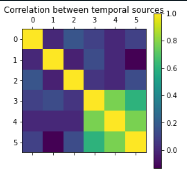
\includegraphics[]{corr tc.png}
    \caption{Correlation matrix}
    \label{fig:corr tc}
\end{figure}
From Figure \ref{fig:corr tc}, we observe that there is high pairwise correlation between three temporal sources (third, fourth and fifth). It can not be easily differentiated which pair (either between third and fourth one or between fourth and fifth one) has higher correlation from the CM. But these two pair has highest correlation.

\subsection{}
\begin{figure}[H]
    \centering
    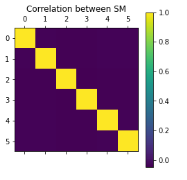
\includegraphics[]{corr tm.png}
    \caption{Correlation matrix}
    \label{fig:corr tm}
\end{figure}
From Figure \ref{fig:corr tm}, it is observed that there is no correlation between these SM indicating independence among them.

\subsection{}
\begin{figure}[H]
\begin{subfigure}{.5\textwidth}
  \centering
  % include first image
  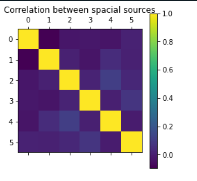
\includegraphics[width=1\linewidth]{corr ts.png}  
  \label{fig:sub-first}
\end{subfigure}
\begin{subfigure}{.5\textwidth}
  \centering
  % include second image
  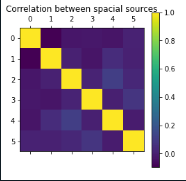
\includegraphics[width=1\linewidth]{corr tt.png}  
  \label{fig:sub-second}
\end{subfigure}

\newline

\begin{subfigure}{.5\textwidth}
  \centering
  % include third image
  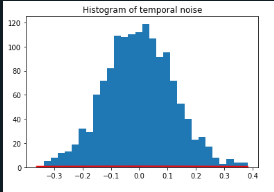
\includegraphics[width=1\linewidth]{hist tt.png}  
  \label{fig:sub-third}
\end{subfigure}
\begin{subfigure}{.5\textwidth}
  \centering
  % include fourth image
  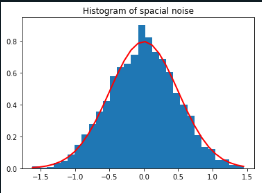
\includegraphics[width=1\linewidth]{ts hist.png} 
  \label{fig:sub-fourth}
\end{subfigure}
\label{fig:all}
\end{figure}

From four above figure of temporal and spacial noises, we observe that these sources are not correlated and both type of noises follow normal distribution.

\begin{figure}[H]
    \centering
    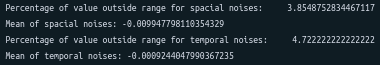
\includegraphics[]{1.4 output.png}
    \caption{Output from notebook}
    \label{fig:corr tm}
\end{figure}

Based on Python output above, these two distribution has approximately fulfilled both mean and variance condition of normal distribution. Despite some violation, this is a very small percentage and can not be fixed due to randomness.

\begin{figure}[H]
    \centering
    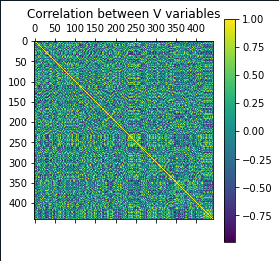
\includegraphics[]{corr V var.png}
    \caption{Output from notebook}
    \label{fig:corr V var}
\end{figure}
From Figure \ref{fig:corr V var}, overall, across 441 variables, the color indicates there is high proportion of correlated variables

\subsection{}
\begin{figure}[H]
    \centering
    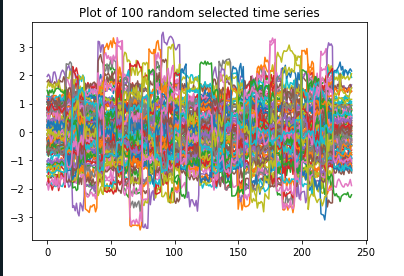
\includegraphics[]{100 temp.png}
    \label{fig:hist var}
\end{figure}

\begin{figure}[H]
    \centering
    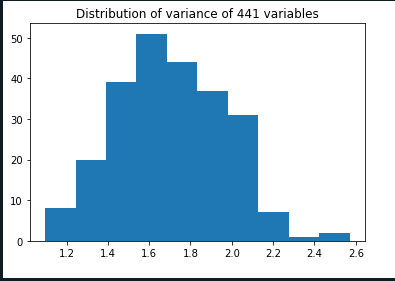
\includegraphics[]{hist var.png}
    \caption{Output from notebook}
    \label{fig:hist var}
\end{figure}
Overall, distribution of variance among variables follows approximate normal distribution, ranging from 1.2 to 2.6. Therefore, it is necessary to standardise the dataset to make the variables equally importance.

\section{Question 2}

\end{document}
